%Appendix_A

%\appendixnodots   %this command is needed here, do not remove it

%%%%%%%%%%%%%%%%%%%%%%%%%%%%%%%%%%%%%%%%%%%%%%%%%%%%%%%%%%%%%%%%%%%%%%%%%%%%%%%%%%%%%%%%%%%%%%%%%%%
%%% Note: Name your appendix A, or B, or C, etc., but don't name it "APPENDIX A", etc. as the word
%%% APPENDIX will be automatically added in the name of the appendix in the text but it won't be
%%% added in the Table of Contents where it will appear only as A, B, C, etc., followed by the title.
%%% This is per new Grad School regulation as of January 2002.
\appendname{Appendix A: \\ \bigskip Harmonically Aligned Signal Projection Interpolation Type}  
\appendix
\label{appendix:Harmonically Aligned Signal Projection Interpolation Type Appendix}                       

In addition to the HASP-D algorithm, an additional method can be utilized for aligning independent carrier frequency harmonics.  Instead of decimating progressively higher rows of frequency bins to realign harmonically related signals, an interpolation method can be utilized to realign harmonics as well.  The frequency bins comprising the row of the highest frequency harmonic, $K$, and bandwidth, $B$, provide the maximum number of bins around the highest harmonic.  Therefore, interpolating the frequency bins within $k \times (f_c \pm B)$, where $k$ is the harmonic number from $k = 1 \ldots K-1$ and $f_c$ is the carrier frequency, by the maximum number of bins around the highest harmonic, $K$, realigns independent carriers.  The HASP Interpolation type (HASP-I) algorithm is described in more detail in Algorithm \ref{alg:haspialg}.

\begin{algorithm}
	\caption{HASP-I Algorithm} \label{alg:haspialg}
	\scriptsize
	\begin{algorithmic}[1]
		\Require~~
		\Statex $\hat{r}$ - Input Power Spectrum
		\Statex $f_c$ - Center Frequency 
		\Statex $B$ - Bandwidth
		\Ensure~~
		\Statex $\bf{H}$ - HASP-I Output Array
		\Statex
		\For  {$k = 1, 2, \ldots K$} 
		\State    $\mathbf{f}_k \gets \left[ \hat{r}(x_i) \right], k(f_c - B/2) \leq x_i \leq k(f_c + B/2)$
		\State		$k$-th row of $\mathbf{H} \gets$ INTERPOLATION $\mathbf{f}_k$ by factor of $\frac{K}{k}$
		\EndFor
	\end{algorithmic}
\end{algorithm}

Although the HASP-D algorithm provides a method for aligning harmonics and modulation sidebands, frequency resolution is lost at higher harmonics due to the decimation process.  The HASP-I algorithm was developed to vertically align the harmonics of independent signals regardless of the chosen center frequency or amount of frequency offset between the carriers and retain the resolution of the higher harmonic bin separation.  The HASP-I algorithm is illustrated in Figure \ref{fig:haspi_diagram_independent}, where each progressive harmonic row is interpolated to a fixed number of bins, based on the number of bins around the highest harmonic, to realign independent harmonics.  Although independent carriers and their respective harmonics align vertically, modulation sidebands ``curve'' in toward the higher harmonics as the bandwidth around the lower harmonic frequencies is expanded out to a larger number of bins through the interpolation process, as shown in Figure \ref{fig:haspi_diagram_modulation}.

\begin{figure}[tp]
	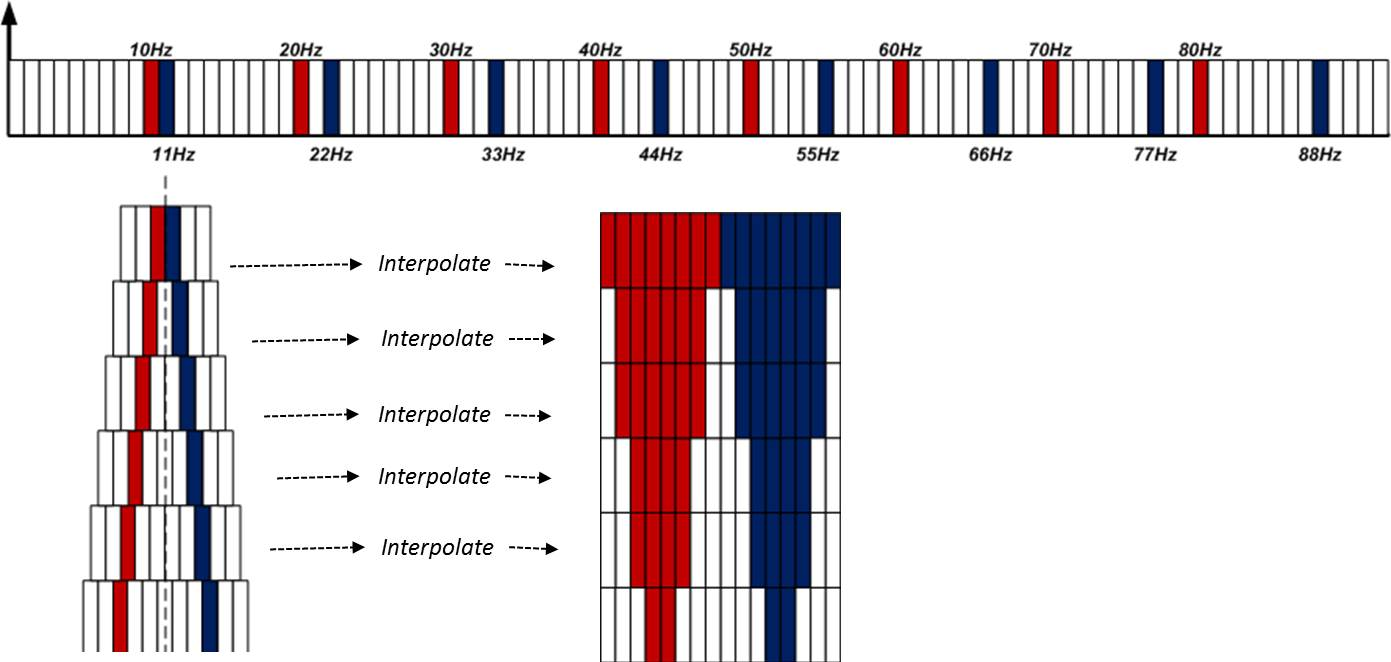
\includegraphics[width=\textwidth]{./misc_graphics/haspi_diagram_independent.jpg}
	\centering
	\caption{Diagram of the HASP-I process applied to a two independent carriers at $10$Hz and $11$Hz with harmonic content, as represented by the red and blue blocks, respectively.  As each harmonic row is added, the number of bins is interpolated to equal the number of bins around the maximum harmonic, $K$, thus aligning the independent carriers.}
	\label{fig:haspi_diagram_independent}
\end{figure}

\begin{figure}[tp]
	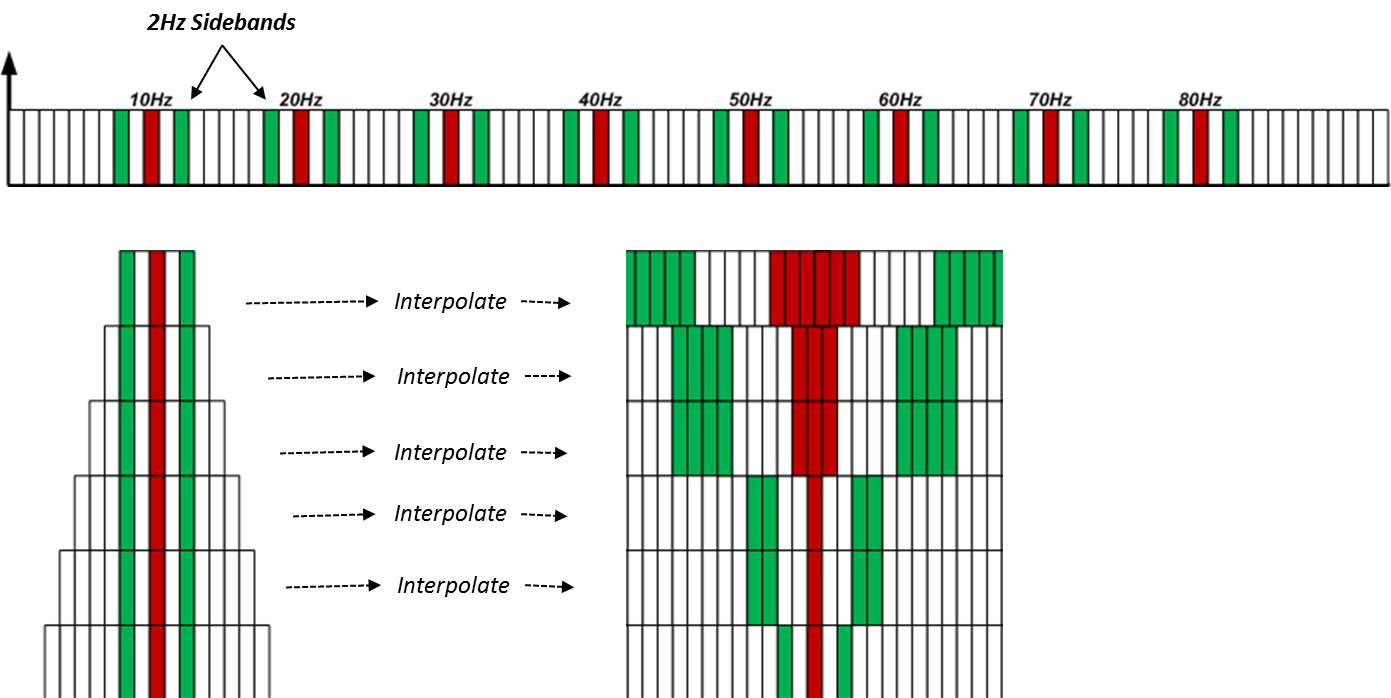
\includegraphics[width=\textwidth]{./misc_graphics/haspi_diagram_modulation.jpg}
	\centering
	\caption{Diagram of the HASP-I process applied to a carrier at $10$Hz with $2$Hz modulation sidebands, as represented by the red and green blocks, respectively.  As each harmonic row is added, the number of bins is interpolated to equal the number of bins around the highest harmonic, $K$, thus causing the modulation sidebands to expand at lower harmonics.}
	\label{fig:haspi_diagram_modulation}
\end{figure}
